% mitz.tex
%
% summary of the Mitzenmacher result for BFs.
\label{sec:mitz}
\newcommand{\hashfam}{\setfont{H}}
\newcommand{\sizes}{\setfont{N}}
\newcommand{\length}{m}
\newcommand{\hashes}{k}
\newcommand{\FP}{\procfont{fp}}
\def\vin(#1,#2){#1 sub}

\begin{figure}[t]
  \centering
  \hspace*{-8pt}
  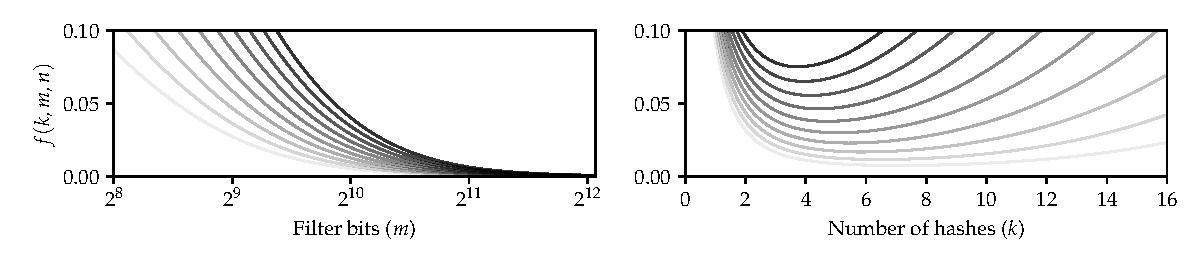
\includegraphics[page=1,scale=0.625]{fig/bf-viz}
  \vspace{-24pt}
  \caption{
    Function $f(k,m,n) = (1-e^{-kn/m})^k$ for various values of~$k$,
    $m$, and $n$.
    %
    In both plots, darker lines are for larger set sizes ($n$); values
    range from $n=100$ to~$200$.
    \textbf{Left:} varying filter length ($m$) and $k=4$ (the number
    of hash functions used in Squid).
    %
    \textbf{Right:} varying number of hashes ($k$) and $m=1024$.
    %
  }
  \vspace{6pt}
  \hrule
  \label{fig:bf-viz}
\end{figure}

This appendix summarizes the results of Kirsch and
Mitzenmacher~\cite{kirsch2006less} for the false-positive probability of Bloom
filters using double hashing.
%
Our presentation is less general than theirs, but suffices for understanding the
results in our paper.

\newcommand{\mset}{\procfont{mset}}
\newcommand{\hashscheme}{\capgreekfont{\Gamma}}
\heading{Additional notation.}
%
If~$\vv$ is a vector, then let~$\mset(\vv)$ denote the multiset comprised of its
elements.
%
Following~\cite{kirsch2006less}, if~$\setM$ is a multiset, we write $i,i
\in \setM$ to mean that~$i$ appears in~$\setM$ at least twice.

\heading{Hashing schemes.}
%
Let~$\elts$ be a set. A \emph{hashing scheme}~$\hashscheme$ for~$\elts$ is a
quadruple $(\hash, \length, \hashes, \sizes)$.
%
The last element is an infinite set $\sizes \subseteq \N$ denoting the permitted
\emph{set sizes}. (We do not require that $\sizes = \N$.)
%
Functions $\length$ and~$\hashes$ specify the filter length~$\length(n)$ and
number of hashes~$\hashes(n)$ respectively for set size~$n$.
%gq
The first element is a function~$\hash\colon\N\by\elts\to\N^*$ mapping a
parameter~$n\in\sizes$ and $x\in\elts$ to a $\hashes(n)$-vector of natural
numbers, which represent bit locations in a filter of length~$\length(n)$.
%
Formally, for every $n \in \sizes$, $\hash(n,\cdot)$ is a random function
specifying a joint distribution on a collection of random variables $\{
\hash(n,x)\colon x\in\elts\}$.
%
We associate to~$\hashscheme$, set~$\col\subseteq\elts$, and
$z\in\elts\setminus\col$ a \emph{false positive event}, denoted
$\FP(\col,z)$, which occurs if for every $j \in [\hashes(n)]$ there
exists some $x\in\col$ such that $\vv_j \in \mset(\hash(n,x))$, where $\vv =
\hash(n,z)$ and $n = \setlen{\col}$.

Fix a set~$\elts$ and a hashing scheme~$\hashscheme = (\hash, \length, \hashes,
\sizes)$ for~$\elts$.  Fix $z\in\elts$ and a collection of subsets $\{ \col_n
\}_{n\in\sizes}$ of $\elts$, where $z\not\in\col_n$ and $\setlen{\col_n} = n$
for each $n \in \sizes$.
%
The following says that, if~$\hashscheme$ satisfies certain conditions, the
false positive probability converges to the approximate bound
of~\cite{broder2004network} as~$n$ increases.
%
\begin{theorem}[Lemma 4.1 of~\cite{kirsch2006less}]
  \label{thm:mitz1}
  Suppose there exist $\lambda, k\in\N$ and a function $\gamma(n) \in o(1/n)$ such
  that for every $n \in \sizes$, it holds that
  \begin{enumerate}
    \item $\hashes(n) = k$;
    \item $\length(n) = O(n)$;
    \item $\{\hash(n, x)\colon x\in\elts\}$ are independent and
      identically distributed;

    \item for every $x \in \elts$, it holds that
      \[
        \max_{i\in\length(n)} \left|
          \Prob{ i \in \mset(\hash(n, x)) } - \lambda/kn
        \right| = O(\gamma(n)) \,;
      \]

    \item and for every $x \in \elts$, it holds that
      \[
        \max_{i,j\in\length(n)}
          \Prob{ i,j \in \mset(\hash(n, x)) } = O(\gamma(n)) \,.
      \]
  \end{enumerate}
  %
  Then $\lim_{n\goesto\infty} \Prob{\FP(\col_n,z)=1} = \left(1 -
  e^{-\lambda/k}\right)^k$.
\end{theorem}
%
Kirsch and Mitzenmacher prove that the \emph{double hashing scheme} defined by
\[
  \hash(n,x)_j = 1 + (h_1(n,x) + j\cdot h_2(n,x) \mod m(n)) \,,
\]
for each $j\in[k]$, where $k(n)=k$ and $m(n)=cn$ for some constants~$k$ and $c$, and
$h_1(n,\cdot)$ and~$h_2(n,\cdot)$ are independent and identically distributed
random functions with range $[m(n)]$, satisfies the conditions of
Theorem~\ref{thm:mitz1} for $\lambda = k^2/c$ and $\gamma(n) = 1/n^2$. (See
\cite[Thorem 5.2]{kirsch2006less}.) Thus, the false-positive probability
converges to $(1-e^{-k/c})^k$ as~$n\goesto\infty$.
%
But how close to this limit is the false positive probability for some
fixed~$n$? To address this question, Kirsch and Mitzenmacher provide an analysis
of the rate of convergence.
%
\begin{theorem}[Theorem 6.1 of~\cite{kirsch2006less}]\label{thm:mitz2}
  Suppose~$\hashscheme$ satisfies the conditions of Theorem~\ref{thm:mitz1}
  for~$\lambda$, $k$, and~$\gamma(n)$. For every~$n\in\sizes$, it holds that
  \[
    \left|
      \Prob{\FP(\col_n,z)=1} - \left(1 - e^{-\lambda/k}\right)^k
    \right| = O(n\gamma(n) + 1/n) \,.
  \]
\end{theorem}
%
For the double hashing scheme in particular, we have that the false positive
probability is at most
$
  (1 - e^{-k/c})^k + O(1/n)
$
for any $n\in\sizes$. (See~\cite[Theorem 6.2]{kirsch2006less}.)

Fix integers $k,m,n,\lambda \geq 0$ and let $H \colon \bits^* \to [m]^k$ and $F
\colon \bits^\lambda\by\bits^*\to[m]^k$ be functions.
%
Let $\struct_\saltybloom = \SBF[\hashbf[H],k,m,n,\lambda]$ and $\struct_\prfbloom =
\SKBF[\hashlin[F],k,m,n,\lambda]$ as defined in Figure~\ref{fig:bf-prf}.
%
If~$H$ and~$F$ are random functions, then $\hashbf[H]$ and $\hashlin[F]$ are
both realizations of the double hashing scheme for a particular choice of~$n$.
%
From Thoerem~\ref{thm:mitz2} it follows that the false positive probability
for~$\struct_\saltybloom$ and~$\struct_\prfbloom$ is at most
$
  (1 - e^{-kn/m})^k + O(1/n).
$
(See Figure~\ref{fig:bf-viz} for a visualization of this bound.)
%
In the proof of security for~$\struct_\saltybloom$
(Theorem~\ref{thm:bf-salt-correct}), we model~$H$ as a random oracle;
%
for~$\struct_\prfbloom$ (Theorem~\ref{thm:bf-prf-correct}), we can treat~$F$ as
a random function assuming it is a good PRF.
